\documentclass[tikz]{standalone}
\usepackage{pgfplots}
\pgfplotsset{compat=1.15}
\usepackage{mathrsfs}
\usetikzlibrary{arrows,calc}
\usepackage{tkz-euclide}
\pagestyle{empty}

\definecolor{AngleClr}{rgb}{0,0.39215686274509803,0}
\definecolor{ShapeClr}{rgb}{0.6,0.2,0}
\definecolor{SquareClr}{RGB}{250, 248, 217}

\begin{document}

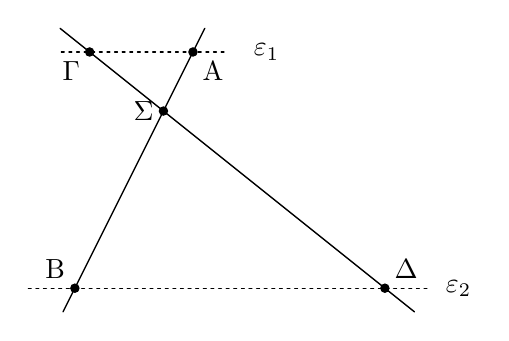
\begin{tikzpicture}[scale=.75]
\tkzSetUpLine[line width=1pt,color=black]
\tkzSetUpPoint[fill=black]

\tkzDefPoints{0/0/S,0.5/1/A,-1.5/-3/B,-1.25/1/C,3.75/-3/D}

\tkzDrawPoints[size=3](A,B,C,D,S)

\tkzDrawSegments[line width=0.5pt,color=black,dashed,dash pattern=on 1pt off 1.75pt,add=0.3 and 0.3](A,C)
\tkzDrawSegments[line width=0.5pt,color=black,dashed,dash pattern=on 1pt off 1.75pt,add=0.15 and 0.15](B,D)
\tkzDrawSegments[line width=0.5pt,color=black,add=0.1 and 0.1](C,D A,B)


\tkzLabelPoint[below right](A){$\rm A$}
\tkzLabelPoint[above left](B){$\rm B$}
\tkzLabelPoint[below left](C){$\rm \Gamma$}
\tkzLabelPoint[above right](D){$\rm \Delta$}
\tkzLabelPoint[left](S){$\rm \Sigma$}

\tkzLabelPoint[right=0.65cm](A){$\varepsilon_1$}
\tkzLabelPoint[right=0.65cm](D){$\varepsilon_2$}

\end{tikzpicture}

\end{document}
